\documentclass[11pt,a4paper]{article}
\usepackage[margin=22mm]{geometry}
\usepackage{graphicx,booktabs,amsmath}
\renewcommand{\thefigure}{S\arabic{figure}}
\renewcommand{\thetable}{S\arabic{table}}
\setcounter{table}{2}\setcounter{figure}{8}
\title{Supplementary material: Four-layout fine-sizing comparison}
\author{Working manuscript review11}\date{19 November 2026}
\begin{document}\maketitle
The four cases retain the best actually evaluated extra-coarse layout at each screened rib count. Spar positions are fixed during independent fine sizing. All cases start from 10~mm total thickness and use the same $R=0.30$~m filter, source aerodynamic loading, full-integration shell formulation, section settings and sizing rules. The completed two-rib result is compared with the unchanged saved 8-, 16- and 25-rib results. No solver calculations were run during manuscript preparation.

Table~\ref{tab:mass} separates final mass into the stress-sized mass and the subsequent reinforcement increment. The two-rib design is lightest among these four fine-sized layouts, despite being the heaviest screening winner. This establishes neither a global optimum nor fine-mesh optimality of the retained spar positions.
\begin{table}[h]\centering\small
\caption{Mass components and maximum total thickness.}\label{tab:mass}
\begin{tabular}{rrrrrr}\toprule
Ribs & Screening (kg) & FSD (kg) & Added (kg) & Final (kg) & Max. total (mm)\\\midrule
2 & 461.147 & 341.373 & 141.763 & 483.136 & 150.000\\
8 & 370.305 & 301.368 & 333.897 & 635.265 & 116.892\\
16 & 372.029 & 308.842 & 239.664 & 548.506 & 117.895\\
25 & 389.145 & 312.889 & 297.771 & 610.661 & 112.815\\
\bottomrule\end{tabular}\end{table}

Table~\ref{tab:effort} reports solved-state counts and measured effort. Each phase count includes its initial state. The two-rib FSD stage stops by feasible mass stagnation; the final buckling correction is uniform-core restoration triggered by near-feasible stagnation. Wall times exclude geometry preparation and final archival.
\begin{table}[h]\centering\small
\caption{Complete-sizing effort and termination.}\label{tab:effort}
\begin{tabular}{rrrrrl}\toprule
Ribs & FSD states & Buckling states & Solver min & Wall min & FSD stop\\\midrule
2 & 103 & 23 & 86.78 & 89.25 & Mass stagnation\\
8 & 23 & 43 & 65.87 & 67.16 & Mass stagnation\\
16 & 24 & 33 & 78.04 & 79.61 & Mass stagnation\\
25 & 8 & 35 & 94.56 & 96.16 & Active fraction\\
\bottomrule\end{tabular}\end{table}

The two-rib model has root and tip ribs and no intermediate ribs. Its raw peak is 497.73~MPa; maximum individual-face thickness is 26.74~mm, with core and total maxima at 100 and 150~mm. Acceptance applies to the adopted filtered-stress and linear-buckling criteria. Systems integration, manufacturing and local-strength requirements remain unassessed. The 16-rib reference studies in the main manuscript do not automatically validate this different candidate.
\clearpage
Figure~\ref{fig:hist} compares the saved histories. The horizontal axis counts solved states through FSD and reinforcement; buckling factors are evaluated only in the second phase.
\begin{figure}[h]\centering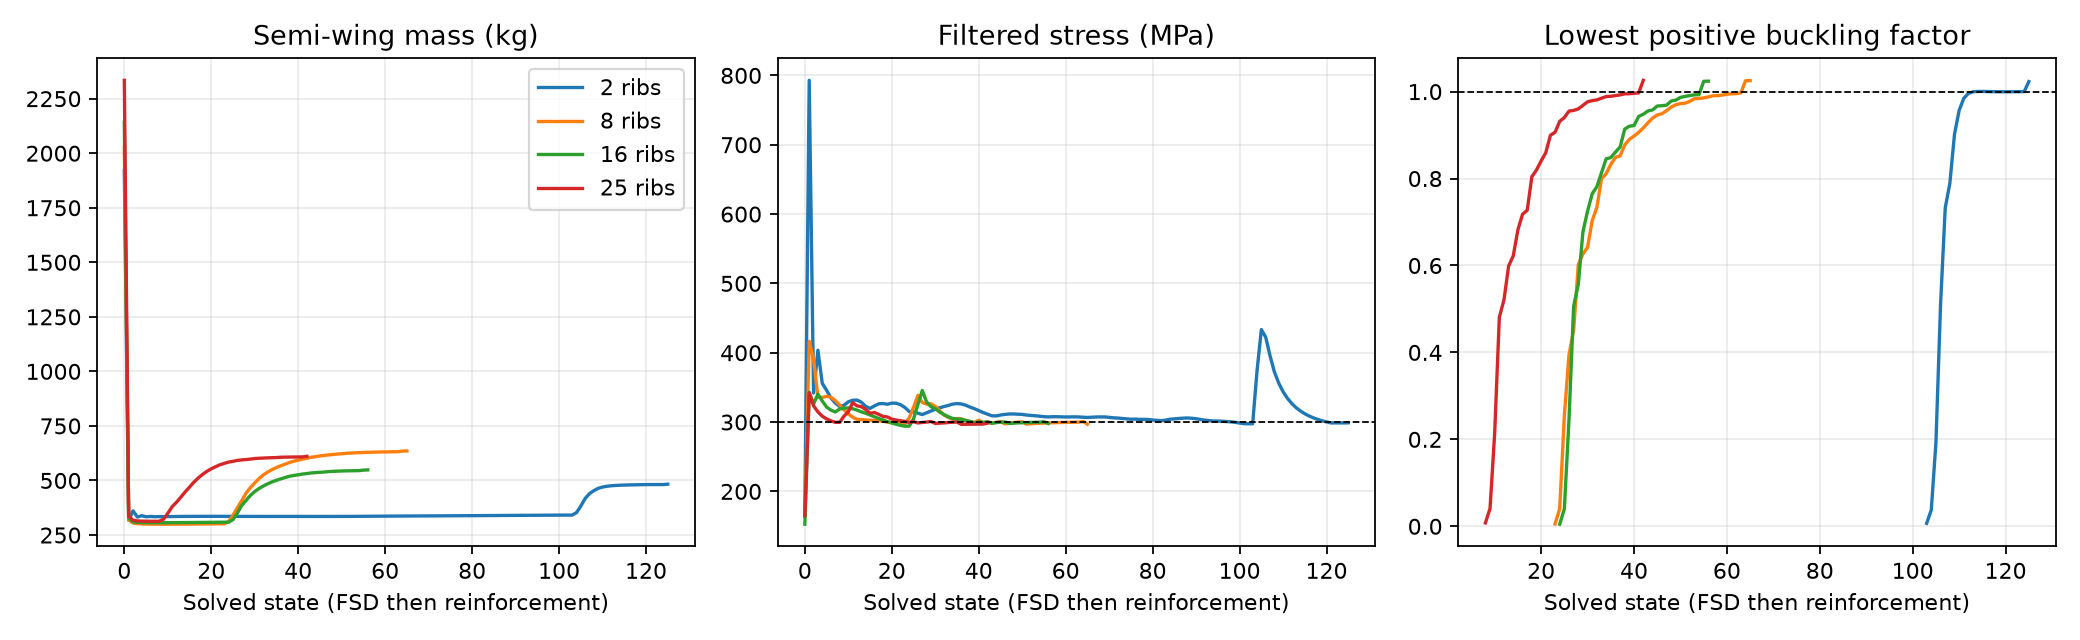
\includegraphics[width=\textwidth]{sizing_histories.png}
\caption{Saved sizing histories for all four fine layouts. Dashed lines mark the filtered-stress and buckling acceptance limits.}\label{fig:hist}\end{figure}
\clearpage
Figure~\ref{fig:mass} displays the mass components in Table~\ref{tab:mass}. The reinforcement increments include the complete grow-only procedure and any stress repair or restoration.
\begin{figure}[h]\centering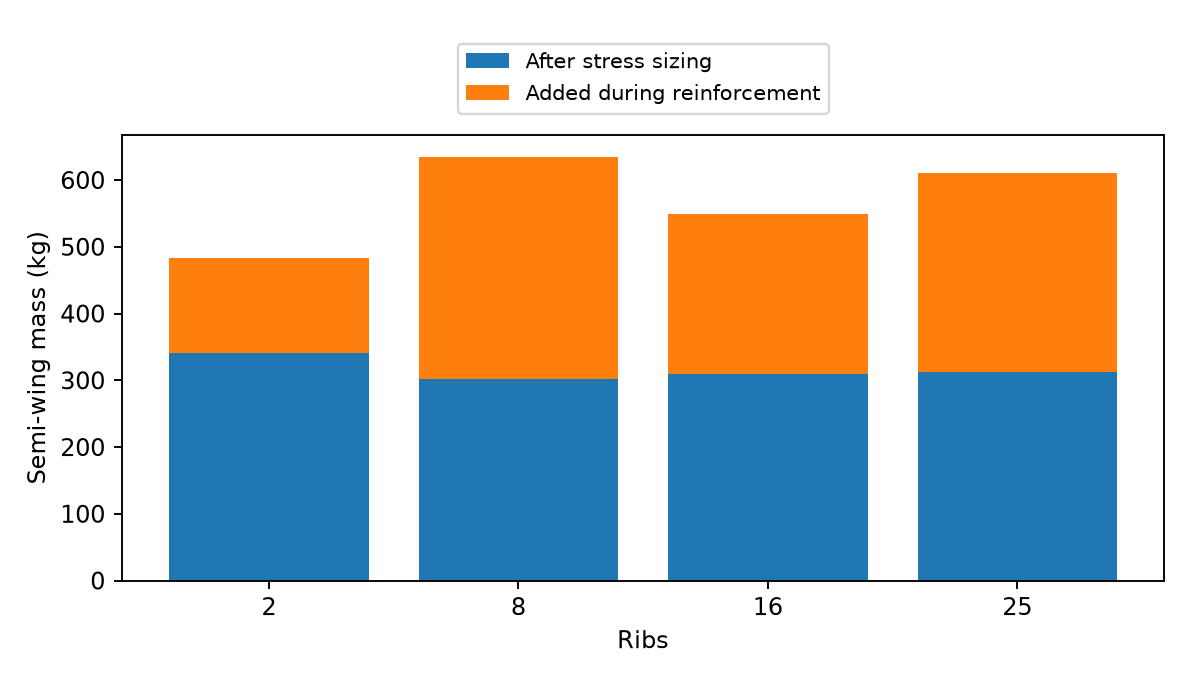
\includegraphics[width=\textwidth]{mass_comparison.png}
\caption{Final semi-wing mass separated into stress-sized mass and subsequent reinforcement.}\label{fig:mass}\end{figure}
\end{document}
